\documentclass[17pt]{beamer}
\usetheme{Madrid}
\usepackage[utf8]{inputenc}
\usepackage[czech]{babel}
\usepackage[T1]{fontenc}
\usepackage{amsmath}
\usepackage{amsfonts}
\usepackage{amssymb}
\usepackage{graphicx}
\author{David Žáček}
\title[Volby do PSP ČR]{Analýza voleb do Poslanecké sněmovny Parlamentu ČR}
%\setbeamercovered{transparent} 
\usepackage{array}
\newcolumntype{L}[1]{>{\raggedright\let\newline\\\arraybackslash\hspace{0pt}}m{#1}}
\newcolumntype{C}[1]{>{\centering\let\newline\\\arraybackslash\hspace{0pt}}m{#1}}
\newcolumntype{R}[1]{>{\raggedleft\let\newline\\\arraybackslash\hspace{0pt}}m{#1}}
\setbeamertemplate{navigation symbols}{} 
\institute{8.M} 
\date{7. března 2017} 
%\subject{} 
\begin{document}

\begin{frame}
\titlepage
\end{frame}

%\begin{frame}
%\tableofcontents
%\end{frame}

\begin{frame}{Úvod}
\center
\begin{block}{Úloha}
Rozdělte $N$ volených funkcí mezi strany účastnící se voleb tak, aby poměr zisku funkcí co nejlépe odpovídal poměru získu hlasů.
\end{block}
\bigskip
\begin{center}
\begin{tabular}{|c|c|c|c|c|c|c|}
\hline
Hlasy & 4700 & 1600 & 1590 & 1200 & 600 & 310  \\ \hline
\end{tabular}
\end{center}
\end{frame}

\begin{frame}{Úvod}
\center
Pro $N=10$:
\bigskip
\begin{center}
\begin{tabular}{|c|c|c|c|c|c|c|}
\hline
Hlasy & 4700 & 1600 & 1590 & 1200 & 600 & 310  \\ \hline
Podíl & 4.7  & 1.6  & 1.59 & 1.2  & 0.6 & 0.31 \\ \hline
      & 5    & 2    & 2    & 1    & 0   & 0    \\ \hline
      & 5    & 2    & 1    & 1    & 1   & 0    \\ \hline
      & 4    & 2    & 2    & 1    & 1   & 0    \\ \hline
\end{tabular}
\end{center}
\end{frame}

\begin{frame}{Počátky poměrných systémů}
\begin{center}

\includegraphics[scale=0.2]{zdroje/const.jpg}
\end{center}
\end{frame}

\begin{frame}{Bez určeného počtu}
%Q"9000/11000		O1"20000	O2"100000
\begin{itemize}
\item Předem zvolené: $Q$
\item Počet hlasu pro stranu: $H_{x}$
\item Zisk mandátů: $\left\lfloor\frac{H_{x}}{Q}\right\rfloor$
\end{itemize}
\end{frame}

\begin{frame}{Metoda nejvyšších zbytků}
\begin{itemize}
\item Počet rozdělovaných mandátů $N$
\item $Q=\dfrac{H_{c}}{N}$
\item Zisk mandátů: $\left\lfloor\frac{H_{x}}{Q}\right\rfloor+\{0;1\}$
\end{itemize}
\end{frame}

\begin{frame}{Paradox nových států}
\begin{center}
\begin{tabular}{|c|c|c|c|}
\hline 
100 k. & Hlasy & Ku kvótě & Křesla \\ 
\hline 
A & 8955 & \hspace{0.35cm}8955/100=89.55\hspace{0.35cm} & 90 \\ 
\hline 
B & 1045 & 1045/100=10.45 & 10 \\ 
\hline 
\end{tabular}
\end{center} 
\begin{center}
\begin{tabular}{|c|c|c|c|}
\hline 
105 k. & Hlasy & Ku kvótě & Křesla \\ 
\hline 
A & 8955 & 8955/100.14=89.42 & 89 \\ 
\hline 
B & 1045 & 1045/100.14=10.44 & 11 \\ 
\hline 
C & 515 & 515/100.14=5.14 & 5 \\ 
\hline 
\end{tabular} 
\end{center}
\end{frame}

\begin{frame}{Alabamský paradox}
\begin{center}
\begin{tabular}{|c|c|c|c|c|c|}
\hline 
 &  & \multicolumn{2}{c|}{10 křesel} & \multicolumn{2}{c|}{11 křesel} \\ 
\hline 
 & Hlasy & Poměr & Zisk & Poměr & Zisk \\ 
\hline 
A & 300 & 4,286 & 4 & 4,714 & 5 \\ 
\hline 
B & 300 & 4,286 & 4 & 4,714 & 5 \\ 
\hline 
C & 100 & 1,426 & 2 & 1.571 & 1 \\ 
\hline
\end{tabular} 
\end{center}
\end{frame}

\begin{frame}{Metody nejvyšších průměrů}
\begin{itemize}
\item Počet rozdělovaných mandátů $N$
\item Zisk mandátů: $\left\langle\frac{H_{x}}{Q}\right\rangle$
\item $\langle$\hspace{0.15cm}$\rangle$ je zaokrouhlení.
\item $Q$ je určeno tak, aby bylo rozděleno \\ právě $N$ křesel.
\end{itemize}
\end{frame}

\begin{frame}{MNP 2 -- spektrum}
\begin{itemize}
\item D'Hondtova metoda $\left\lfloor\frac{H_{x}}{Q}\right\rfloor$
\item Metoda Sainte-Lague $\left\lfloor\frac{H_{x}}{Q}\right\rfloor$
\item Adamsova Metoda $\left\lceil\frac{H_{x}}{Q}\right\rceil$
\item Metoda Huntington-Hill: zaokrouhlení dle geometrického průměru.
\end{itemize}
\end{frame}

\begin{frame}{MNP 3 -- výpočet řadou}
\begin{itemize}
\item Běžně se počíta pomocí řady \uv{mezí zaokrouhlení}
\item Pro zaokrouhlení dolu (D'Hondt) je řada $1; 2; 3; 4; ...$
\item Pro zaokrouhlení běžné (Sainte-Lague) je řada $0{,}5; 1{,}5; 2{,}5; 3{,}5; ...$
\\ nebo také ekvivalentní $1; 3; 5; 7; ...$
\end{itemize}
\end{frame}

\begin{frame}{Příklad D'Hondtovy metody}
\begin{itemize}
\item A:49, B:45, C:18
\item Pro 6 křesel:
\end{itemize}
\begin{center}
\begin{tabular}{|C{2cm}|C{2cm}|C{2cm}|C{2cm}|}
\hline 
 & A & B & C \\ 
\hline 
1 & \textbf{49} & \textbf{45} & \textbf{18} \\ 
\hline 
2 & \textbf{24,5} & \textbf{22,5} & 9 \\ 
\hline 
3 & \textbf{16,33} & 15 & 6 \\ 
\hline 
4 & 12,25 & 11,25 & 4,5 \\ 
\hline 
\end{tabular} 
\end{center}
\end{frame}

\begin{frame}{Hypotetické volby}
\begin{itemize}
\item 200 poslanců
\item Tři strany A, B, C
\item A:49\%, B:45\%, C:6\%
\item Homogenně rozložená podpora
\end{itemize}
\end{frame}

\begin{frame}{Výsledky}
\begin{center}
\begin{tabular}{|l|c|c|c|} \hline
  & A & B & C \\ \hline 
Přesný poměr & 98 & 90 & 12\\ \hline
\end{tabular}
\end{center} 
\end{frame}

\begin{frame}{Výsledky}
\begin{center}
\begin{tabular}{|l|c|c|c|} \hline
  & A & B & C \\ \hline 
Přesný poměr & 98 & 90 & 12\\ \hline
SR & 98 & 90 & 12\\ \hline
\end{tabular}
\end{center} 
\end{frame}

\begin{frame}{Výsledky}
\begin{center}
\begin{tabular}{|l|c|c|c|} \hline
  & A & B & C \\ \hline 
Přesný poměr & 98 & 90 & 12\\ \hline
SR & 98 & 90 & 12\\ \hline
ČR & 102 & 94 & 3\\ \hline
\end{tabular}
\end{center} 
\end{frame}

\begin{frame}{Výsledky}
\begin{center}
\begin{tabular}{|l|c|c|c|} \hline
  & A & B & C \\ \hline 
Přesný poměr & 98 & 90 & 12\\ \hline
SR & 98 & 90 & 12\\ \hline
ČR & 102 & 94 & 3\\ \hline
UK/USA & 200 & 0 & 0\\ \hline
\end{tabular}
\end{center} 
\end{frame}

\begin{frame}{Výsledky}
\begin{center}
\begin{tabular}{|l|c|c|c|} \hline
  & A & B & C \\ \hline 
Přesný poměr & 98 & 90 & 12\\ \hline
SR & 98 & 90 & 12\\ \hline
ČR & 102 & 94 & 3\\ \hline
UK/USA & 200 & 0 & 0\\ \hline
\end{tabular}
\end{center} 
V roce 2006 opravdu získala Strana zelených $6{,}29\%$ hlasu ale jen $3\%$ poslanců. 
\textbf{Jak je to možné?}
\end{frame}

\begin{frame}{Kraje}
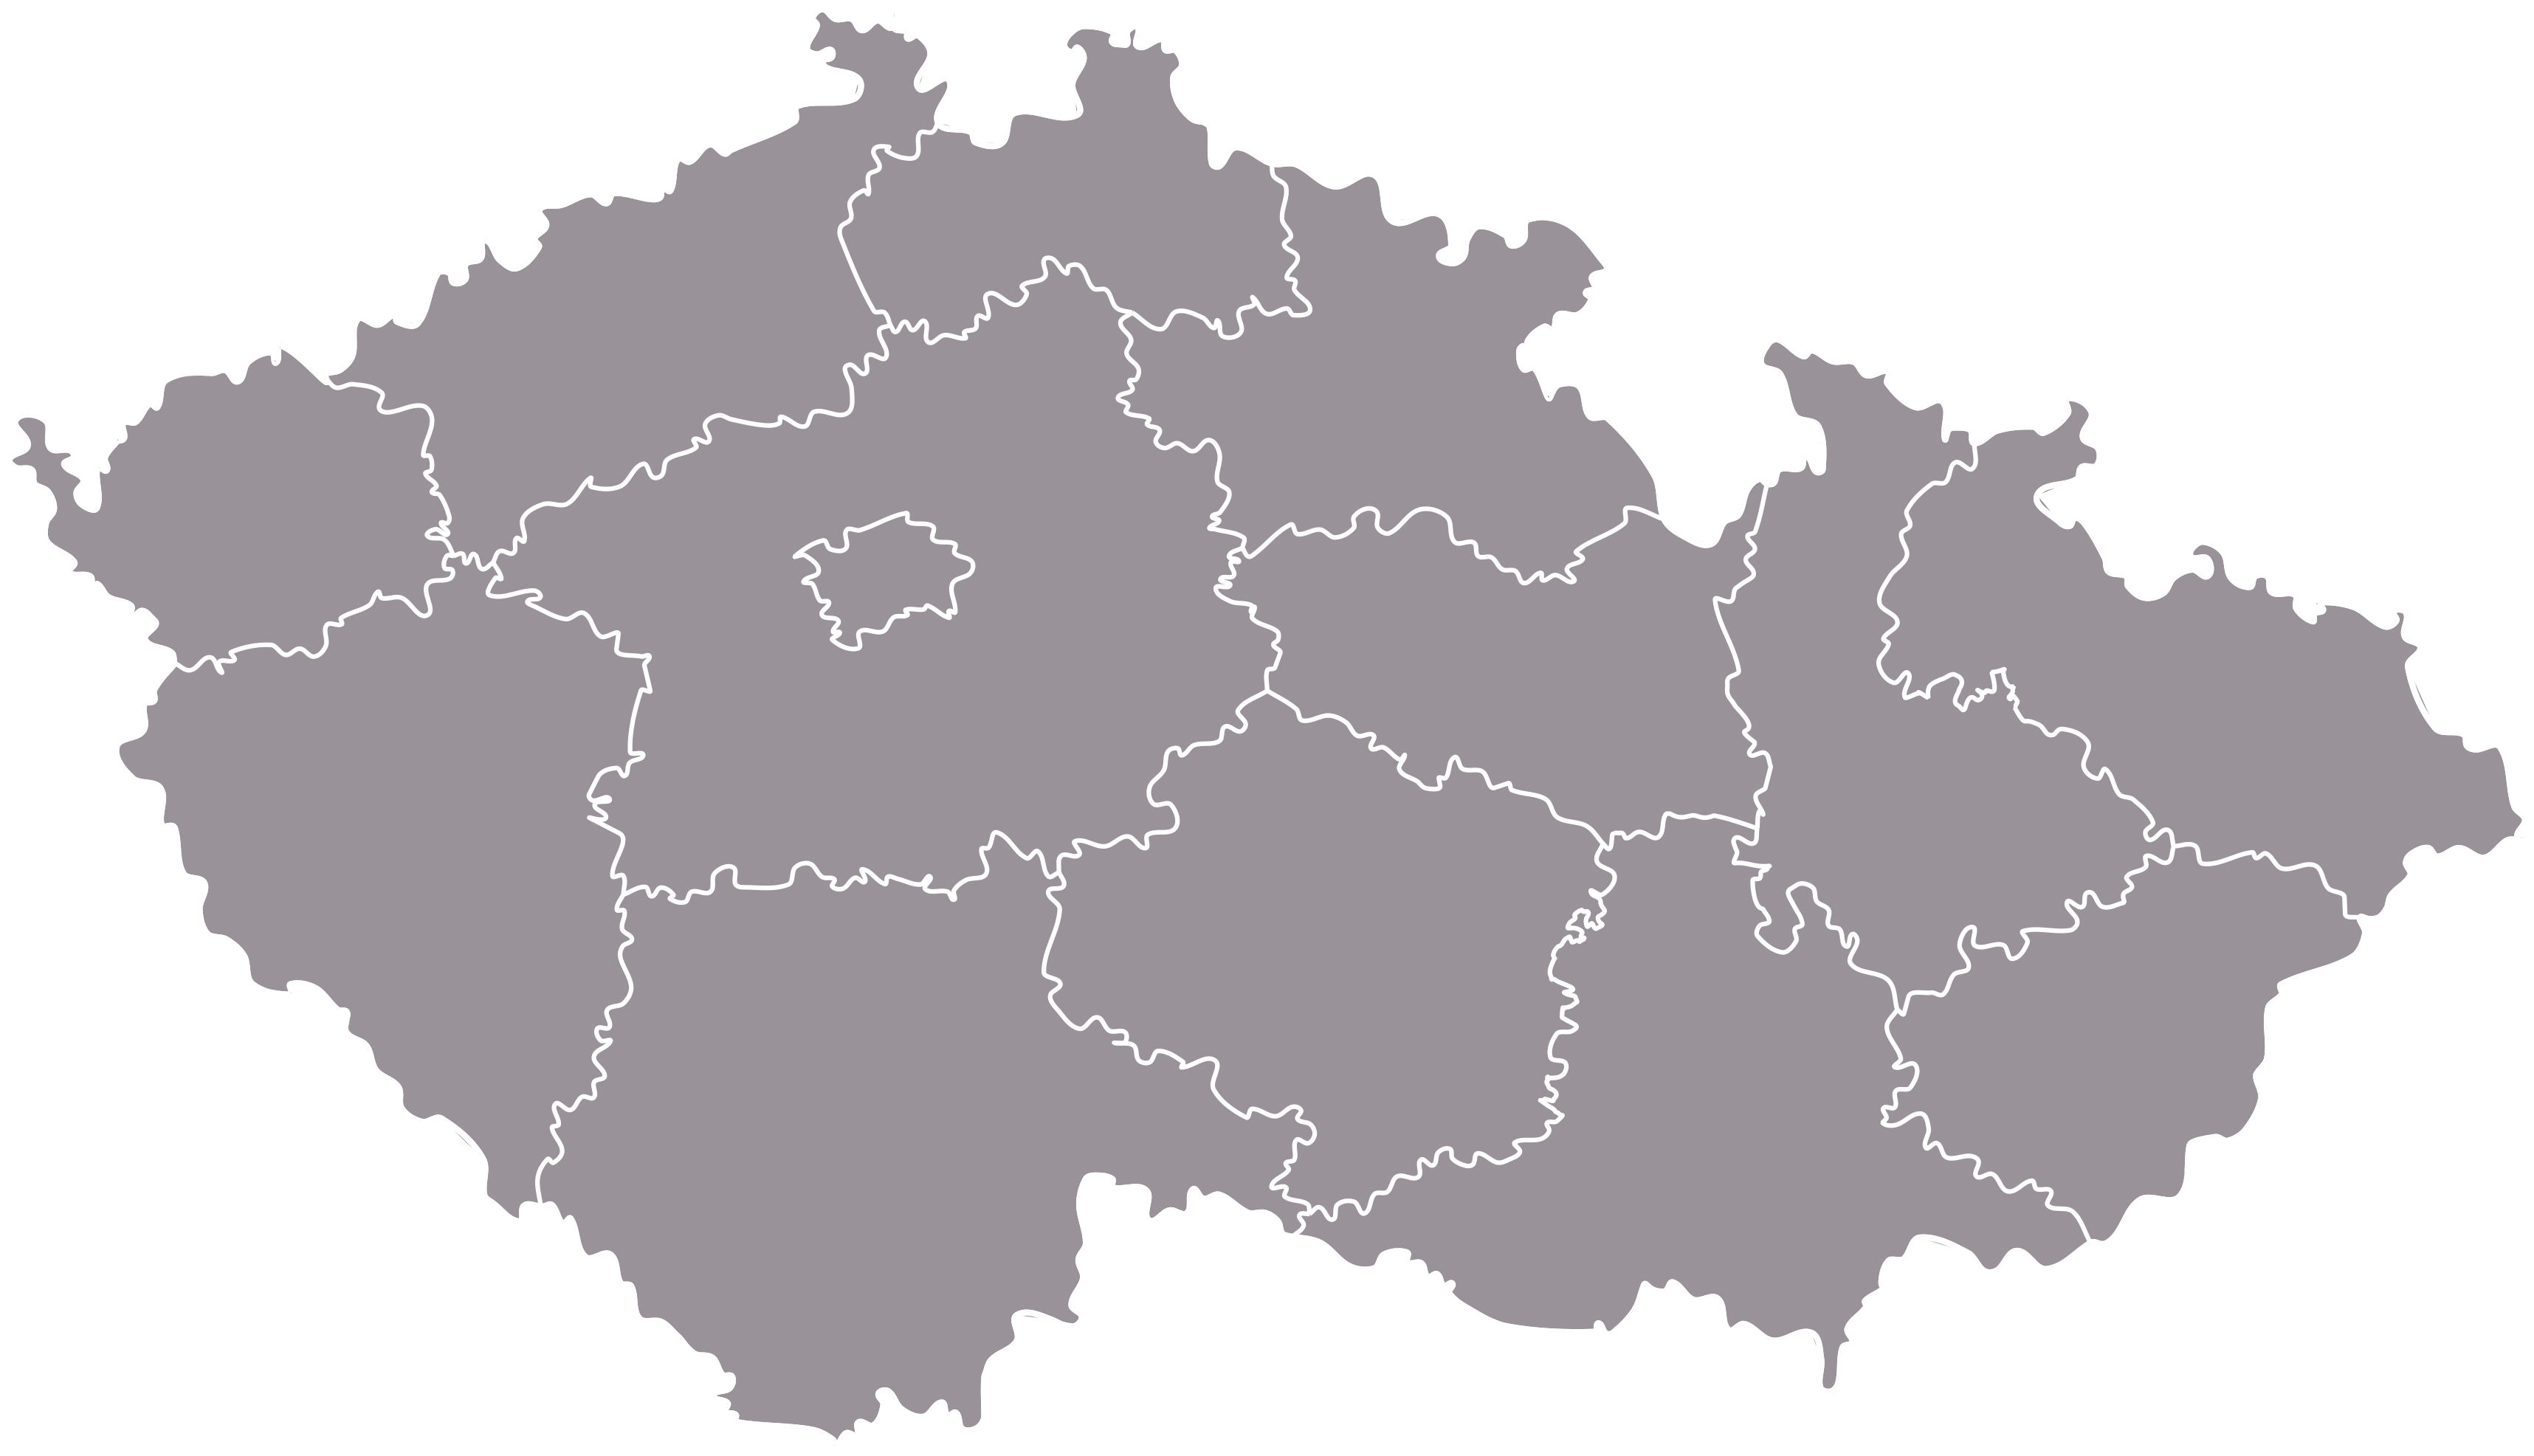
\includegraphics[scale=0.1]{zdroje/kraje.png}
\end{frame}

\begin{frame}{Karlovarský kraj (5) 2006 a 2013}
\begin{center}
\begin{tabular}{|c|c|}
\hline
Strana  & Zisk    \\ \hline
ODS     & 38,33\% \\ \hline
ČSSD    & 34,98\% \\ \hline
SZ      & 7,17\%  \\ \hline
KSČM    & 15,84\% \\ \hline
KDU-ČSL & 3,68\%  \\ \hline
\end{tabular}
\begin{tabular}{|c|c|}
\hline
Strana  & Zisk    \\ \hline
ČSSD    & 24,28\% \\ \hline
TOP09   & 11,47\% \\ \hline
ODS     & 7,65\%  \\ \hline
KDU-ČSL & 3,82\%  \\ \hline
Úsvit   & 9,48\%  \\ \hline
ANO2011 & 24,25\% \\ \hline
KSČM    & 19,02\% \\ \hline
\end{tabular}
\end{center}
\end{frame}

\begin{frame}{Kraje -- reseni}

\end{frame}

\begin{frame}{Konec hlaseni}

\end{frame}

https://www.census.gov/population/apportionment/about/history.html

\end{document}
